\section{Theorie}
Der Dampfdruck $p^*$ ist der Druck einer gasförmigen Komponente, der sich im Gleichgewicht über einer Flüssigkeit einstellt.
Er ist insbesondere bei reinen Flüssigkeiten und Abwesenheit anderer gasförmigen Komponenten leicht zu messen.
Wird der Druck in Abhängigkeit der Temperatur aufgezeichnet, so ergibt sich die sogenannte Dampfdruckkurve, einer der Bestandteile des Phasendiagramms einer Substanz.
Sie beginnt am Tripelpunkt der Substanz, an dem alle drei Aggregatszustände zeitgleich existieren, und endet am kritischen Punkt, ab welchem die Grenze zwischen flüssig und gasförmig vollständig verschwinden.

Die thermodynamische Beschreibung der Dampdruckkurve folgt aus der Gibbs-Energie für einen reinen Stoff.
\begin{equation*}
    \odif{G} = \pdv{G}{T}_{V} \odif{T} + \pdv{G}{V}_{T} \odif{p} = - S\odif{T} + V\odif{p}
\end{equation*}
Es wird die Veränderung des Dampfdrucks für veränderliche Temperaturen betrachtet.
Die Steigung der Dampfdruckkurve ist dann gegeben durch
\begin{equation*}
    \odv{p}{T} = \frac{S_g - S_l}{V_g - V_l} = \adv{S}{V} = \adv{S_m}{V_m}
\end{equation*}
Es handelt sich bei Phasenübergängen generell um einen reversiblen Prozess. Somit kann die molare Entropie $\Delta S_m$ durch die Verdampfungsenthalpie $\Delta H_m$ sowie die Verdampfungstemperatur $T$ ersetzt werden.
Ferner ist das molare Volumen $V_m$ eines Gases ein sehr deutliches Vielfaches des molaren Volumen der Flüssigkeit, es kann $V_{m,l}$ vernachlässigt werden.
Zusätzlich dient als Näherung des molaren Volumens das ideale Gasgesetz.
Für den Versuch relevant ist die hieraus folgende Clausius-Clapeyron-Gleichung, deren Integration dann einen exponentiellen Zusammenhang liefert.
\begin{align}
    \Delta V_m &\approx V_{m,g} \approx \frac{RT}{p} \nonumber \\
    \odv{p}{T} &= \frac{p \Delta H_m}{RT^2} \nonumber \\
    \Rightarrow p^*(T_2) &= p^*(T_1) \exp\left( \frac{\Delta H_m}{R}\left( \frac{1}{T_1} - \frac{1}{T_2} \right) \right) \label{eqn:clausius-clapeyron}
\end{align}
Zur Auswertung werden basierend auf diesem Zusammenhang die gemessenen $p$ gegen $\frac{1}{T}$ aufgetragen.

\section{Durchführung}

\begin{figure}[H]
    \centering
    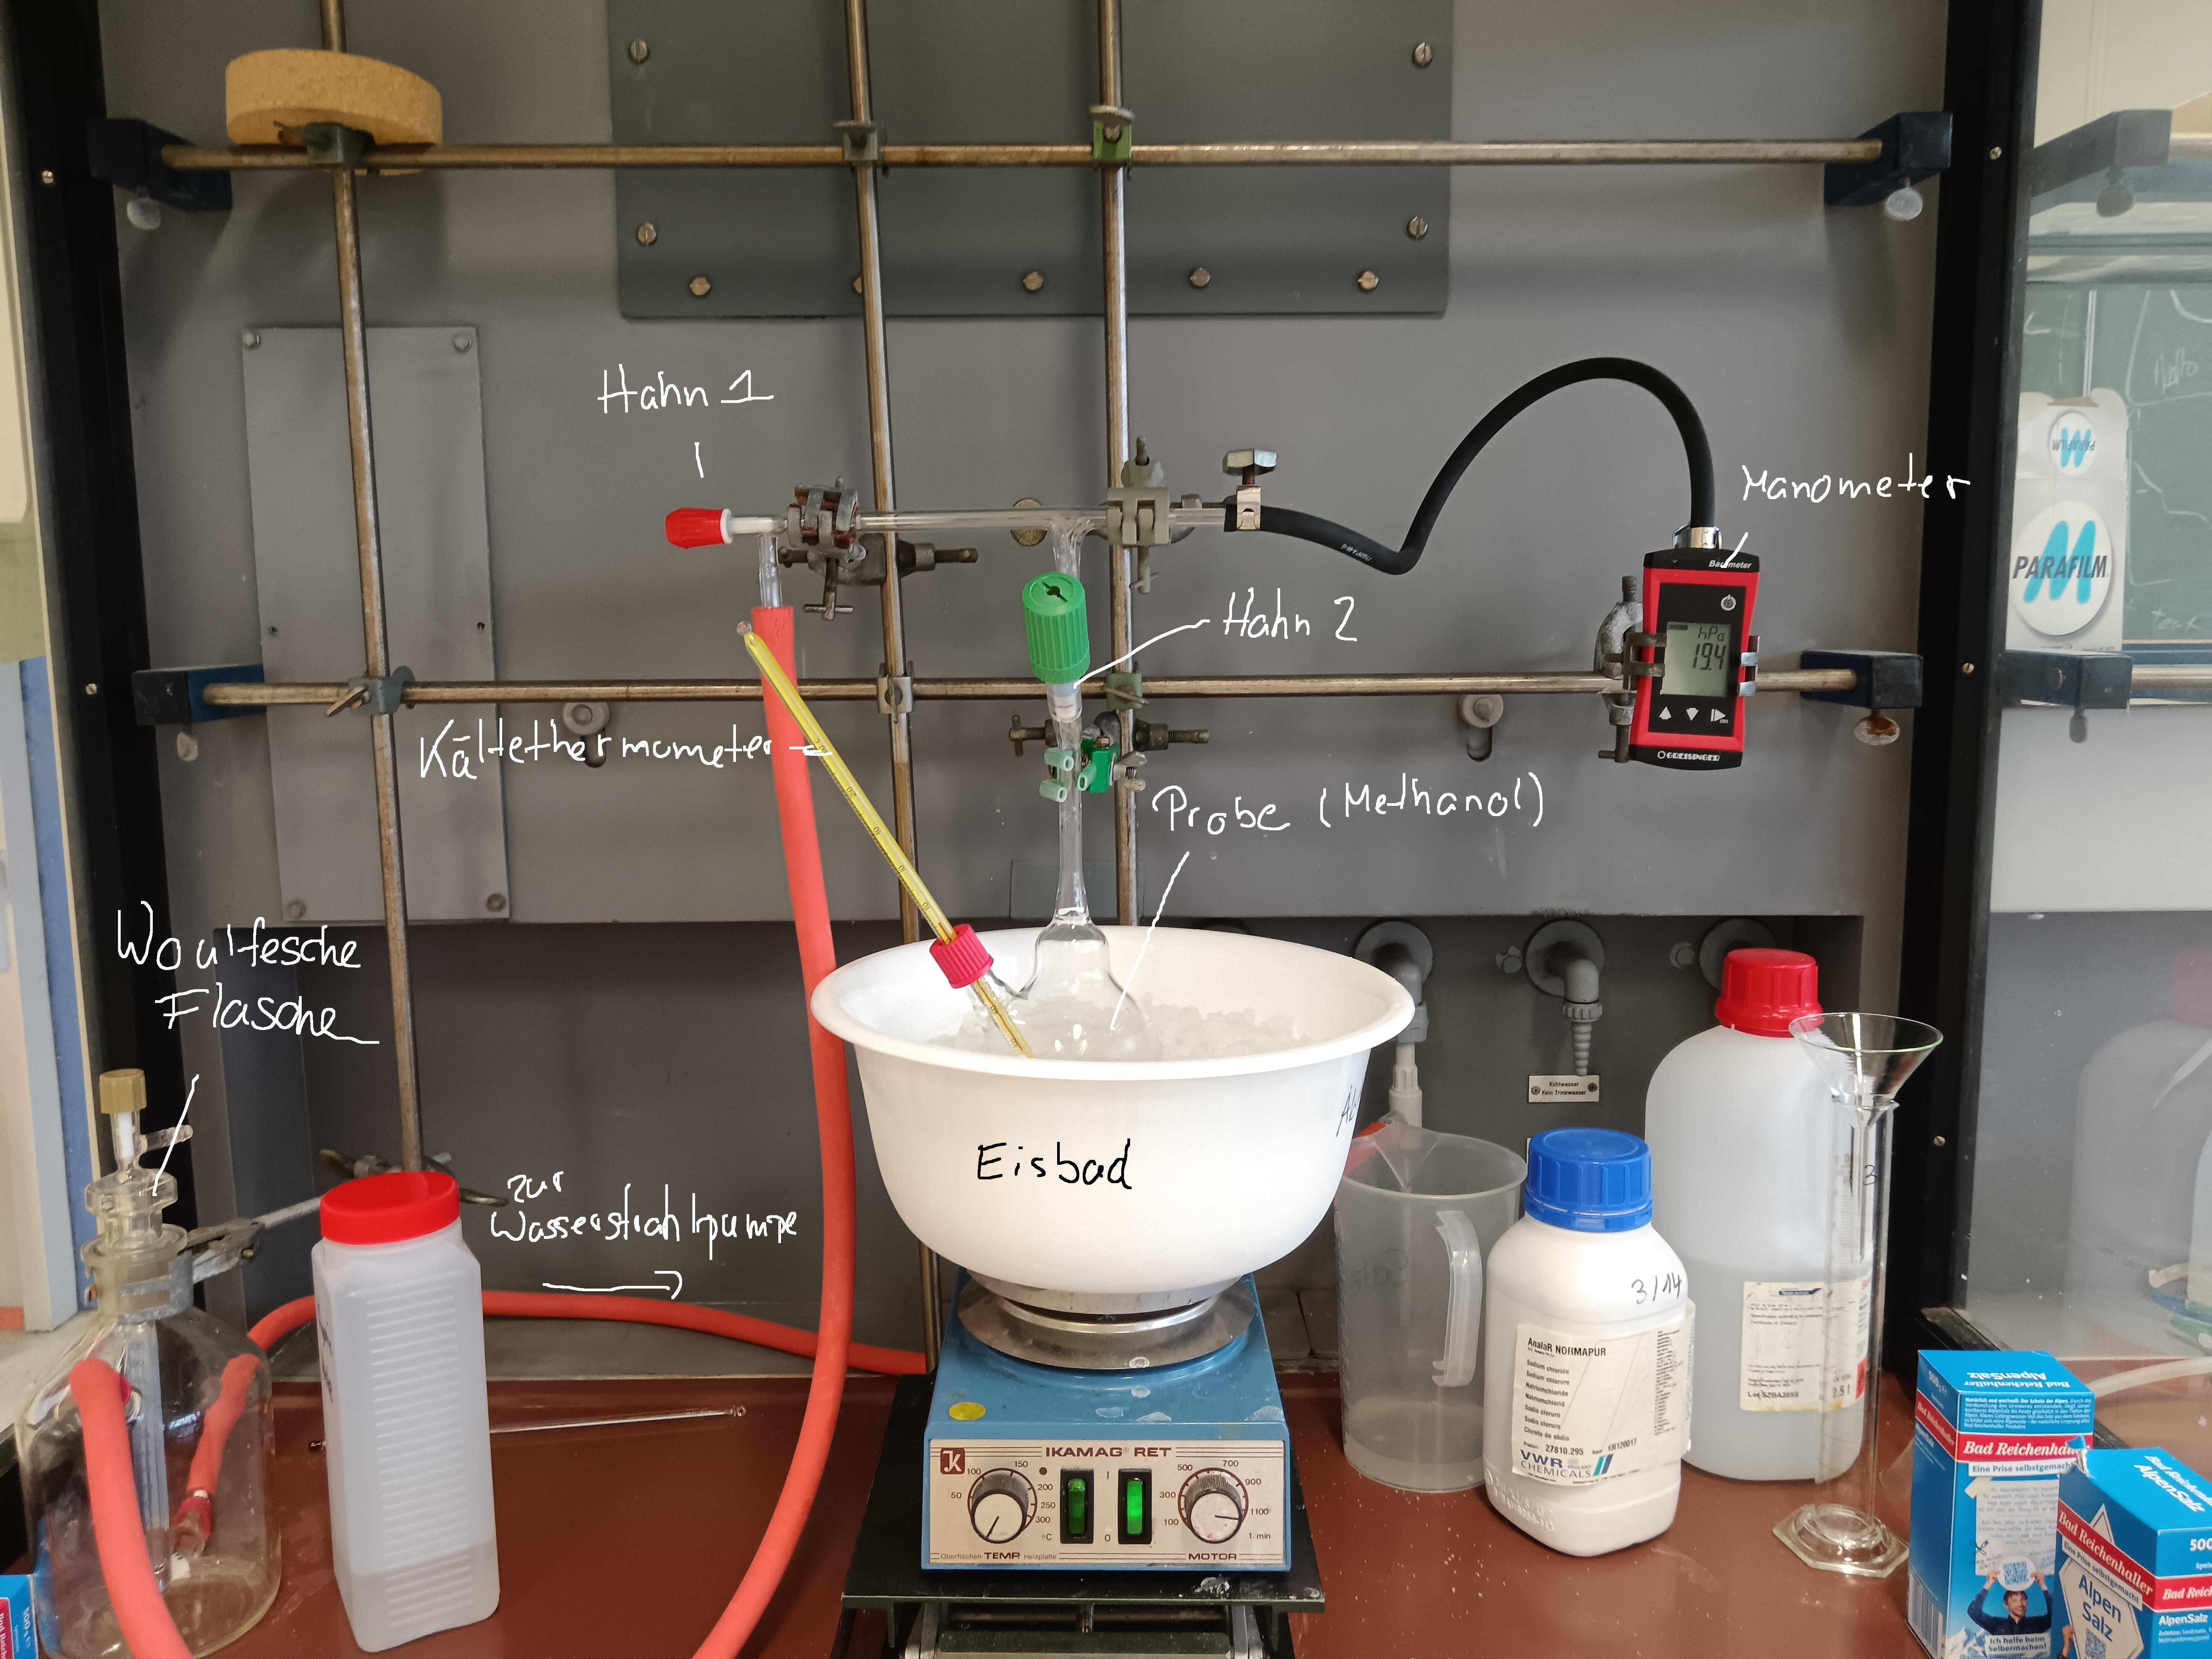
\includegraphics[width=\linewidth]{T2/Versuchsaufbau_annotated.jpg}
    \caption{\textbf{Versuchsaufbau}.
        Hahn 1 war über die Woulfesche Flasche mit der Wasserstrahpumpe verbunden.
        Die Probe wurde durch Hahn 2 vom direkten Weg zur Pumpe isoliert.
        Der Probe wurden einige Siedesteinchen hinzugegeben, um einem Siedeverzug vorzubeugen, zusätzlich wurde die Probe durch den Magnetrührer gerührt.
        }
    \label{fig:versuchsaufbau}
\end{figure}

\subsection{Vorbereitung}
Hahn 1 am Glasaufbau wurde geschlossen und die Wasserstrahlpumpe bereits am Vortag vom Betreuer gestartet.
Eine Kältemischung von zwei Teilen Eis und einem Teil Kochsalz wurde angesetzt und in einer Schale bereitgehalten.
Zur Evakuierung des Aufbaus wurde Hahn 2 geöffnet, geschlossen, dann Hahn 1 wieder geöffnet.
Dieser Vorgang wurde dreimal wiederholt.

Die Schale mit der Kältemischung wurde auf den Laborboy gestellt und dieser hoch gefahren, sodass die Flüssigkeit im Rundkolben vollständig von der Kältemischung umgeben ist.
Die Flüssigkeit wurde etwa \qty{10}{\minute} unter Rühren abgekühlt.
Die Evakuierung wurde anschließend dreimal wiederholt, sodass Hahn 1 geschlossen und Hahn 2 geöffnet war.

\subsection{Messung}
Nach Abkühlen der Flüssigkeit wurde die Kältemischung durch Herunterfahren des Laborboys entfernt.
Während des Erwärmens der Flüssigkeit wurden in Abständen von etwa \qty{2}{\kelvin} die Temperatur und der Druck notiert.
Beim Annähern an die Raumtemperatur wurde durch Handwärme unterstützt.
Die Messung wurde insgesamt zweimal durchgeführt.
Zwischen den Messungen wurde zuerst wieder gekühlt, dann dreimal evakuiert.

Am Ende des Versuches wurde zur Belüftung der Apparatur Hahn 1 geschlossen, das Ventil an der Woulfeschen Flasche geöffnet, die Wasserstrahlpumpe gestoppt, und dann Hahn 1 und 2 geöffnet.

\section{Auswertung und Diskussion}
\subsection{Vergleich der Druck- und Temperaturunsicherheiten}
Während die Genauigkeit des Manometers durch die letzte Nachkommastelle des digitalen Displays fest vorgegeben ist, muss der Fehler $\Delta p^{*}$ über die Gaußsche Fehlerfortpflanzung nach der Gleichung $\Delta p^{*} = f'(T) \cdot \Delta T$ berechnet werden.
Da der Dampfdruck gemäß der Clausius-Clapeyron-Gleichung exponentiell mit der Temperatur ansteigt, führt bereits eine geringe Temperaturabweichung von $0,5$ K zu einer Druckänderung, die signifikant größer ist als die Anzeigeungenauigkeit des Messgeräts.

Mathematisch lässt sich zeigen, dass dieser durch die Temperatur induzierte Fehler $\Delta p^{*}$ über den gesamten untersuchten Temperaturbereich nahezu konstant bleibt, da die Zunahme der Steigung der Dampfdruckkurve bei höheren Temperaturen die relative Genauigkeit stabilisiert. Siehe hierzu \autoref{sec:err-dampfdruck}.

Die auf Basis der Temperatur ermittelte Unsicherheit des Dampfdruckes von \qty{376.6}{\pascal} übersteigt die Unsicherheit des Manometers von \qty{20}{\pascal} um ein Vielfaches.
Die Unsicherheit des Manometers ist also vernachlässigbar.

\subsection{Genauigkeit des Temperaturermittlung}
Zur Bestimmung der Messunsicherheit muss die Ablesegenauigkeit des verwendeten Kältethermometers kritisch hinterfragt werden.
Das Thermometer wies eine Skalierung auf, die theoretisch eine Ablesegenauigkeit von \textbf{höchstens} \qty{1}{\degreeCelsius} ermöglicht.

Da es sich bei dem Versuch jedoch um eine dynamische Messung handelt, bei welcher die Temperatur während der Aufnahme der Aufheizkurve kontinuierlich ansteigt, treten zusätzliche Unsicherheiten auf.
Hierzu zählen die thermische Trägheit von Methanol sowie die menschliche Reaktionszeit bei der zeitgleichen Erfassung von Druck und Temperatur.

Andererseits kann durch gute Beobachtung der Temperatur das Erreichen der Intervalle bedingt vorhergesagt werden, wodurch ein Anteil der Reaktionszeit und thermischen Trägheit kompensiert werden können.
Unter Berücksichtigung dieser Umstände wird die Unsicherheit der Temperaturermittlung für die weitere Fehlerrechnung auf \qty{0.5}{\kelvin} abgeschätzt.

\subsection{Ermittlung der Verdampfungsenthalpie}
Die Messdaten wurden gemäß der Clausius-Clapeyron-Gleichung
\begin{equation}
\ln \left( \frac{p^*}{p_0} \right) = \frac{\Delta H_{m}}{R} \cdot \left( \frac{1}{T_{S}} - \frac{1}{T} \right)
\end{equation}
aufgetragen, wobei $\ln \frac{p^*}{p_0}$ gegen $\frac{1}{T}$ (in \unit{\per\kelvin}) dargestellt wurde. 
Die Steigung $m$ dieser Geraden entspricht dem Term $- \frac{\Delta H_m}{R}$.

Die ermittelten Ausgleichsgeraden werden beschrieben durch
\begin{align*}
    y_1 &= (\num{-4162.5 +- 462.5})x + (\num{12.2 +- 1.6}) \\
    y_2 &= (\num{-4220.8 +- 506.5})x + (\num{12.4 +- 1.8}) \\
    \implies \bar{y} &= (\num{-4191.7 +- 342.9})x + (\num{12.3 +- 1.2})
\end{align*}
Es folgen somit für die Verdampfungsenthalpie $\Delta H_m$ und der Siedetemperatur $T_S$
\begin{align*}
    \Delta H_m &= -m \cdot R \\
    &= \qty{4191.7 +- 342.9}{\per\kelvin} \cdot \qty{8.314462}{\joule\per\kelvin\per\mol} \\
    &= \qty{34851.7}{\joule\per\mol} = \qty{34.9 +- 2.9}{\kilo\joule\per\mol}
\intertext{Für die Siedetemperatur $T_S$ gilt folgender Zusammenhang}
    \ln \frac{p^*}{p_0} &= \frac{\Delta H_m}{R} \frac{1}{T_S} \\
    T_S &= \frac{\Delta H_m}{R} \frac{1}{\ln \frac{p^*}{p_0}} \\
    &= \frac{\qty{34851.7 +- 2900}{\joule\per\mol}}{\qty{8.314462}{\joule\per\mol\per\kelvin}} \frac{1}{\num{12.3 +- 1.2}} \\
    &= \qty{340.7 +- 43.7}{\kelvin} = \qty{67.55 +- 43.7}{\degreeCelsius}
\end{align*}

Diese Werte stimmen gut mit den Literaturwerten von \qty{35.2}{\kilo\joule\per\mol}\autocite{etde_6190977} und \qty{64.6}{\degreeCelsius}\autocite{crc:methanol} überein.
Allerdings ist die Aussagekraft über den Siedepunkt eher gering, da die Unsicherheit dessen sehr groß ist.

Diese große Unsicherheit der Siedetemperatur resultiert möglicherweise aus systematischen Fehlern, die in der Versuchsdurchführung entstanden sind.
Hierzu zählt beispielsweise eine unzureichende Evakuierung des Aufbaus, wodurch der gemessene Dampfdruck durch Luftdruckanteile verfälscht wurde, oder eine ungenaue Temperaturmessung durch die thermische Trägheit des Thermometers beziehungsweise der Probe.
Ferner ist im angewandten Verfahren die Siedetemperatur abhängig von der Verdampfungsenthalpie.
Wenn also diese bereits durch nicht exakt zeitgleiches Ablesen des Druckes mit Erreichen der gesetzten Temperaturintervalle bestimmt wird, so pflanzt sich dieser Fehler fort und wird verstärkt.

\section{Zusammenfassung}
In diesem Versuch wurde die Dampfdruckkurve von Methanol aufgenommen und ausgewertet.
Hieraus konnten die Verdampfungsenthalpie $\Delta H_m = \qty{34.9 +- 2.9}{\kilo\joule\per\mol}$ und die Siedetemperatur $T_S = \qty{67.55 +- 43.7}{\degreeCelsius}$ bestimmt werden.
Die Verdampfungsenthalpie stimmt gut mit dem Literaturwert von \qty{35.2}{\kilo\joule\per\mol} überein.
Die Unsicherheit der Siedetemperatur ist jedoch sehr groß, was auf systematische Fehler in der Versuchsdurchführung zurückzuführen sein könnte.
Es wurde die Vernachlässigbarkeit der Messunsicherheit des Manometers im Vergleich zur durch die Temperaturunsicherheit induzierten Unsicherheit des Dampfdrucks diskutiert.
Ebenfalls wurde die Ablesegenauigkeit des Thermometers kritisch hinterfragt und eine realistische Unsicherheit von \qty{0.5}{\kelvin} abgeschätzt.

\newpage
\printbibliography
\newpage
\appendix

\section{Fehlerrechnung}
\subsection{Unsicherheit des Dampfdrucks}\label{sec:err-dampfdruck}
Für den Dampfdruck gilt
\begin{equation*}
    p^*(T) = p^0 \cdot \exp{\left(\frac{\Delta H_m}{R} \cdot \left (\frac{1}{T_S} - \frac{1}{T} \right)\right)}
\end{equation*}
Nach Gauß gilt für die Unsicherheit
\begin{equation*}
    \Delta p^* =  \left| \odv{p^*}{T} \right| \cdot \Delta T
\end{equation*}
$T_S$, $R$, $p^0$, und $\Delta H_m$ sind Konstanten. Es folgt für die Ableitung
\begin{align*}
    \odv{p^*}{T} &= p^0 \exp{\left( \frac{\Delta H_m}{R} \cdot \left( \frac{1}{T_S} - \frac{1}{T} \right)\right)} \cdot
                    \underbrace{\odv{}{T} \left[ \frac{\Delta H_m}{R} \cdot \left( \frac{1}{T_S} - \frac{1}{T} \right) \right]}_{\text{Kettenregel}} \\
    &= p^0 \exp{\left( \frac{\Delta H_m}{R} \cdot \left( \frac{1}{T_S} - \frac{1}{T} \right)\right)} \cdot - \frac{\Delta H_m}{RT^2} \\
    \implies \Delta p^* &= \left| p^* * \frac{\Delta H_m}{RT^2} \right| \Delta T
\end{align*}
Für $T = \qty{23}{\degreeCelsius} (= \qty{296.15}{\kelvin})$ der ersten Messung gilt somit
\begin{equation*}
    \Delta p^* = \left| 15880 \cdot \frac{4181.9}{296.15^2} \right| 0.5 \approx \qty{371.44}{\pascal}
\end{equation*}
Für einen Vergleich mit der Messunsicherheit des Manometers wird der Mittelwert aus dieser und der Unsicherheit der zweiten Messung bei der selben Temperatur gebildet.
Es folgt
\begin{equation*}
    \Delta {p}^* = \frac{371.44 + 381.71}{2} = \qty{376.57}{\pascal}
\end{equation*}

\subsection{Verdampfungsenthalpie}
Im verwendeten Verfahren ist die Verdampfungsenthalpie gegeben durch
\begin{equation*}
    \Delta H_m = -m \cdot R
\end{equation*}
Die Unsicherheit $\Delta (\Delta H_m)$ hängt also nur von der Unsicherheit der Steigung $\Delta m$ ab.
Diese ist für die einzelnen Auftragungen gegeben durch die halbe Spanne der Extremgeraden.
Hier beispielhaft für die erste Messung.
\begin{align*}
    \Delta m_1 &= \pm \left| \frac{m_{max,1} - m_{min,1}}{2} \right| \\
    &= \pm \left| \frac{-3700 - (-4625)}{2} \right| \\
    &= \pm 462.5
\end{align*}
Analog dazu wird für die y-Achsenabschnitte der Ausgleichsgeraden verfahren.
Die Unsicherheit der gemittelten Ausgleichsgeraden ist gegeben durch
\begin{align*}
    \overline{\Delta m} &= \frac{1}{N} \cdot \sqrt{ \sum_i \Delta m_i^2} \\
    &= \frac{1}{2} \cdot \sqrt{(\qty{462.5}{\per\kelvin})^2 + (\qty{506.6}{\per\kelvin})^2} \\
    &= \pm \qty{342.9}{\per\kelvin}
\end{align*}
Schließlich wird die Unsicherheit $\overline{\Delta \Delta H_m}$ mittels Gaußscher Fehlerfortpflanzung berechnet.
\begin{align*}
    \overline{\Delta \Delta H_m} &= \sqrt{\left( \pdv{\Delta H_m}{m} \cdot \overline{\Delta m}] \right)^2} \\
    &= \sqrt{\left( - R \cdot \overline{\Delta m} \right)^2} \\
    &= \sqrt{\left( \qty{8.314462}{\joule\per\mol\per\kelvin} \cdot \qty{342.9}{\per\kelvin} \right)^2} \\
    &= \pm \qty{2851.1}{\joule\per\mol} \approx \qty{2.9}{\kilo\joule}
\end{align*}

\subsection{Siedetemperatur}
Für die Siedetemperatur gilt
\begin{equation*}
    T_S = \frac{\Delta H_m}{R} \frac{1}{\ln \frac{p^*}{p_0}}
\end{equation*}
Somit ist die Unsicherheit abhängig von der Unsicherheit in $\Delta H_m$ und des y-Achsenabschnittes.
\begin{align*}
    \Delta T_S &= \sqrt{\left( \pdv{T_S}{\Delta H_m} \cdot \overline{\Delta \Delta H_m} \right)^2 + \left( \pdv{T_S}{y} \cdot \Delta y \right)^2} \\
    &= \sqrt{\left( \frac{1}{Ry} \cdot \overline{\Delta \Delta H_m} \right)^2 + \left( -\frac{\Delta H_m}{Ry^2} \cdot \Delta y \right)^2} \\
    &= \sqrt{\left( \frac{1}{\qty{8.314462}{\joule\per\mol\per\kelvin} \cdot 12.3} \cdot \qty{2851.1}{\joule\per\mol} \right)^2
            + \left( -\frac{\qty{34851.7}{\joule\per\mol}}{\qty{8.314462}{\joule\per\mol\per\kelvin}\cdot 12.3^2} \cdot 1.2 \right)^2} \\
    &= \qty{43.7}{\kelvin}
\end{align*}

\subsection{Fehlerbalken}
Für den Ausdruck $\ln \frac{p^*}{p_0}$ auf der Ordinate wird die Fehlerfortpflanzung auf die logarithmierte Form der Clausius-Clapeyron-Gleichung angewandt.
\begin{align*}
    \Delta \ln \frac{p^*}{p_0} &= \odv{g}{T} \cdot \Delta T \\
\intertext{mit}
    g(T) &= \frac{\Delta H_m}{R} \cdot \left( \frac{1}{T_S} - \frac{1}{T} \right) \\
    \wedge{}\, m &= -\frac{H_m}{R} \\
    \implies \odv{g}{T} &= \frac{m}{T^2} \\
    \implies \Delta \ln \frac{p^*}{p_0} &= \left| \frac{m}{T^2} \right| \Delta T \\
\intertext{Für die erste Messung bei $T = \qty{258.15}{\kelvin}$ folgt}
    \Delta \ln \frac{p^*}{p_0} &= \left| \frac{\qty{4181.9}{\per\kelvin}}{(\qty{258.15}{\kelvin})^2} \right| \cdot \qty{0.5}{\kelvin} \\
    &= 0.031
\intertext{Ebenda, für $T = \qty{296.15}{\kelvin}$}
    \Delta \ln \frac{p^*}{p_0} &= \left| \frac{\qty{4181.9}{\per\kelvin}}{(\qty{296.15}{\kelvin})^2} \right| \cdot \qty{0.5}{\kelvin} \\
    &= 0.0023
\end{align*}

\includepdf[pages=-]{T2/messungen.pdf}
